\documentclass[a4paper,english,10pt,NET]{tumarticle}

% TUM packages
\usepackage{tumfonts}
\usepackage{tumarticle}
\usepackage{tumlocale}
\usepackage{tumcmd}

\usepackage{graphicx} % Required for inserting images
\usepackage[style=american]{csquotes}
\usepackage{hyperref}
\usepackage{xspace}

\usepackage{tabularx}
\usepackage{booktabs}
\usepackage{pdflscape}

\usepackage{siunitx}
\usepackage{todo}

\usepackage{cleveref}

\usepackage{tikz}
\usepackage{messagepassing}
\usepackage{bytefield}
\usetikzlibrary{arrows.meta,calc,fit,positioning,decorations.pathmorphing,automata,shapes}
\tikzset{
	>={Stealth[scale=0.7]},
	every edge/.style={>={Stealth[scale=0.7]},draw,},
	automata/.style={
		->,
		every edge/.style={>={Stealth[scale=1.3]},font=\footnotesize,shorten >=1pt,draw,},
		font=\small,
		initial text={},
		every state/.style={draw=TUMBlue,very thick,fill=TUMLightBlue,ellipse,},
		every loop/.style={looseness=5,},
		node distance=1.8cm and 2.3cm,
	},
}

\renewcommand{\eg}{\mbox{e.\,g.}\xspace} % already defined in tumcmd but without xspace
\renewcommand{\ie}{\mbox{i.\,e.}\xspace} % already defined in tumcmd but without xspace
\newcommand{\cf}{\mbox{c.\,f.}\xspace}
\newcommand{\tos}{$\to$\xspace}

% Set document title. If no language is supplied, the document language is
% assumed.
\title{P2Psec Project -- Midterm Report}
\author{Fabio Gaiba, Lukas Heindl}
\date{July 2nd, 2024}

\begin{document}

\maketitle
\thispagestyle{tumarticle}

\section{Introduction}
% TODO(no one for now)

Let's remember the team name \textbf{Whisper2Peer} :)

\Todo{write later, summary of the rest, not strictly needed but would be nice}

\section{Changes to initial assumptions}
% TODO(Fabio)

\Todo{no substantial changes but few minor ones: no gitlab CI (see moodle), no git hooks yet}

\section{Module Architecture}
% TODO(Fabio)

\Todo{describe highlevel overview}
\begin{figure}
	\centering
	\scalebox{0.75}{
	\newlength\widthV
	\newlength\widthM
	\newlength\widthG
	\newlength\widthH
	\settowidth\widthV{\footnotesize two threads (read+write) per}
	\settowidth\widthM{\footnotesize store which module registered}
	\settowidth\widthG{Gossip-Strategy}
	\settowidth\widthH{\footnotesize two threads (read+write) per}
	\newlength\distance
	\setlength\distance{\dimexpr1.3\linewidth-\widthV-\widthM-\widthG-\widthH-0.34em*8}
	\newlength\myheadsep
	\setlength\myheadsep{.0ex}
	\begin{tikzpicture}[
		node distance=0.33\distance,
		every node/.style={align=left,},
		thick,
		]
		% first create the headers
		\node[text width=\widthV] (v) {Vertical API \hfill (tcp)};
		\node[yshift=-\myheadsep,fit=(v),inner ysep=0pt] (vertAPI) {};

		\node[text width=\widthM,right=of v.north east,anchor=north west,align=center] (m) {Main};
		\node[yshift=-\myheadsep,fit=(m),inner ysep=0pt] (main) {};

		\node[text width=\widthG,right=of m.north east,anchor=north west,align=center] (g) {Gossip-Strategy};
		\node[yshift=-\myheadsep,fit=(g),inner ysep=0pt] (gStrat) {};

		\node[text width=\widthH,right=of g.north east,anchor=north west] (h) {Horizontal API \hfill (tcp)};
		\node[yshift=-\myheadsep,fit=(h),inner ysep=0pt] (horAPI) {};

		% fill the vertical API box
		\coordinate (tmp) at (vertAPI.south);
		\node[anchor=north west,font=\tt] (v1) at (tmp -| vertAPI.west) {
				bind+listen
				\\
				while true:
				\\
				\mbox{    }accept \tos dispatch
			};
		\coordinate (tmp) at (v1.south);
		\path let
			\p1 = ($(vertAPI.west)!0.2!(vertAPI.east)$),
			\p2 = ($(vertAPI.west)!0.5!(vertAPI.east)$),
			\p3 = ($(vertAPI.west)!0.8!(vertAPI.east)$),
			in
			node[anchor=north west,align=center] (t2) at (tmp -| vertAPI.west) {
				\footnotesize
				two threads (read+write) per
				\\
				\footnotesize
				open connection
			}
			coordinate (tmp) at (t2.south)
			coordinate[yshift=-6ex] (end) at (t2.south)
			(\p1 |- tmp) edge[thick,decorate,decoration={snake,amplitude=2pt,segment length=2ex}] (\p1 |- end)
			node[anchor=center] at ($(end)!.5!(tmp)$) {\ldots}
			(\p3 |- tmp) edge[thick,decorate,decoration={snake,amplitude=2pt,segment length=2ex}] (\p3 |- end)
			coordinate (tmp) at (end)
			node[anchor=north] (t3) at (tmp) {
				\footnotesize
				(un)marshal / conn $\leftrightarrow$ main
			}
			coordinate[] (tmp) at (t3.south)
			;
		\coordinate (endV) at (tmp);

		% fill the main box
		\coordinate (tmp) at (main.south);
		\node[anchor=north west,font=\tt] (m1) at (tmp -| main.west) {
				config+setup
				\\
				while true:
				\\
				\mbox{    }filter+relay messages
			};
		\coordinate (tmp) at (m1.south);
		\node[anchor=north west] (m2) at (tmp -| main.west) {
				\footnotesize
				store which module registered
				\\
				\footnotesize
				for what type
			};
		\coordinate[yshift=-1ex] (tmp) at (m2.south);
		\path let
			\p2 = ($(main.west)!0.5!(main.east)$),
			in
			coordinate[yshift=-6ex] (end) at (tmp)
			(\p2 |- tmp) edge[thick,decorate,decoration={snake,amplitude=2pt,segment length=2ex}] (\p2 |- end)
			coordinate (tmp) at (end)
			;
		\coordinate (endM) at (tmp);

		% fill the gossip strategy box
		\coordinate (tmp) at (gStrat.south);
		\node[anchor=north west,font=\tt] (g1) at (tmp -| gStrat.west) {
				while true:
				\\
				\mbox{    }execute strat
				\\
				\hfil\&\&
				\\
				\mbox{    }bookkeeping
			};
		\coordinate (tmp) at (g1.south);
		\node[anchor=north west,text width=\widthG] (g2) at (tmp -| gStrat.west) {
				\footnotesize
				execute the actual strategy, like push or pull
			};
		\coordinate[yshift=-1ex] (tmp) at (g2.south);
		\path let
			\p2 = ($(gStrat.west)!0.5!(gStrat.east)$),
			in
			coordinate[yshift=-6ex] (end) at (tmp)
			(\p2 |- tmp) edge[thick,decorate,decoration={snake,amplitude=2pt,segment length=2ex}] (\p2 |- end)
			coordinate (tmp) at (end)
			;
		\coordinate (endG) at (tmp);

		% fill the horizontal API box
		\coordinate (tmp) at (horAPI.south);
		\node[anchor=north west,font=\tt] (h1) at (tmp -| horAPI.west) {
				connect to neighbors
				\\
				bind+listen
				\\
				while true:
				\\
				\mbox{    }accept \tos dispatch
			};
		\coordinate (tmp) at (h1.south);
		\path let
			\p1 = ($(horAPI.west)!0.2!(horAPI.east)$),
			\p2 = ($(horAPI.west)!0.5!(horAPI.east)$),
			\p3 = ($(horAPI.west)!0.8!(horAPI.east)$),
			in
			node[anchor=north west,align=center] (t2) at (tmp -| horAPI.west) {
				\footnotesize two threads (read+write) per\\
				\footnotesize open connection
			}
			coordinate (tmp) at (t2.south)
			coordinate[yshift=-6ex] (end) at (t2.south)
			(\p1 |- tmp) edge[thick,decorate,decoration={snake,amplitude=2pt,segment length=2ex}] (\p1 |- end)
			node[anchor=center] at ($(end)!.5!(tmp)$) {\ldots}
			(\p3 |- tmp) edge[thick,decorate,decoration={snake,amplitude=2pt,segment length=2ex}] (\p3 |- end)
			coordinate (tmp) at (end)
			node[anchor=north] (t3) at (tmp) {\footnotesize (un)marshal / main $\leftrightarrow$ conn}
			coordinate[] (tmp) at (t3.south)
			;
		\coordinate (endH) at (tmp);

		% determine the max/min coordinates
		\node[fit=(endV) (endM) (endG) (endH)] (end) {};
		\coordinate (end) at (end.south);

		% draw the arrows vert <> main
		\path[every node/.style={font=\footnotesize,},] let
			\p1 = ($(vertAPI.south)!.33!(end)$),
			\p2 = ($(vertAPI.south)!.63!(end)$),
			\p3 = ($(vertAPI.south)!.69!(end)$),
			in
			(\p1 -| vertAPI.east) edge[->] node[above] {vertToMain} (\p1 -| main.west)
			(\p2 -| vertAPI.east) edge[<-] coordinate[pos=0] (a1)  node[above] {mainToVert} (\p2 -| main.west)
			(\p3 -| vertAPI.east) edge[<-] coordinate[pos=1] (a2) (\p3 -| main.west)
			node at ($(a1)!.5!(a2)$) {\ldots}
			;

		% draw the arrows main <> gossip strategy
		\path[every node/.style={font=\footnotesize,},] let
			\p1 = ($(vertAPI.south)!.33!(end)$),
			\p2 = ($(vertAPI.south)!.66!(end)$),
			in
			(\p1 -| main.east) edge[<-] node[above] {stratToMain} (\p1 -| gStrat.west)
			(\p2 -| main.east) edge[->] coordinate[pos=0] (a1)  node[above] {mainToStrat} (\p2 -| gStrat.west)
			;

		% draw the arrows gossip strategy -> hor
		\path[every node/.style={font=\footnotesize,},] let
			\p1 = ($(gStrat.south)!.33!(end)$),
			\p2 = ($(gStrat.south)!.63!(end)$),
			\p3 = ($(gStrat.south)!.69!(end)$),
			in
			(\p1 -| gStrat.east) edge[<-] node[above] {horToStrat} (\p1 -| horAPI.west)
			(\p2 -| gStrat.east) edge[->] coordinate[pos=0] (a1)  node[above] {stratToHor} (\p2 -| horAPI.west)
			(\p3 -| gStrat.east) edge[->] coordinate[pos=1] (a2) (\p3 -| horAPI.west)
			node at ($(a1)!.5!(a2)$) {\ldots}
			;

		% draw the boxes
		\node[inner sep=0pt,fit=(vertAPI.south west) (vertAPI.south east) (end -| vertAPI),draw] (wholeV) {};
		\node[inner sep=0pt,fit=(main.south west) (main.south east) (end -| main),draw] (wholeM) {};
		\node[inner sep=0pt,fit=(gStrat.south west) (gStrat.south east) (end -| gStrat),draw] (wholeG) {};
		\node[inner sep=0pt,fit=(horAPI.south west) (horAPI.south east) (end -| horAPI),draw] (wholeH) {};
	\end{tikzpicture}
}

	\caption{A high level overview of the modules and the channels.}
	\label{fig:overview}
\end{figure}

\subsection{Logical structure}

% TODO(Lukas)
\Todo{class diagram (landscape page)}

\begin{landscape}
	\pagestyle{empty}
	\begin{figure}
		\centering
		\hspace*{-0.1\linewidth}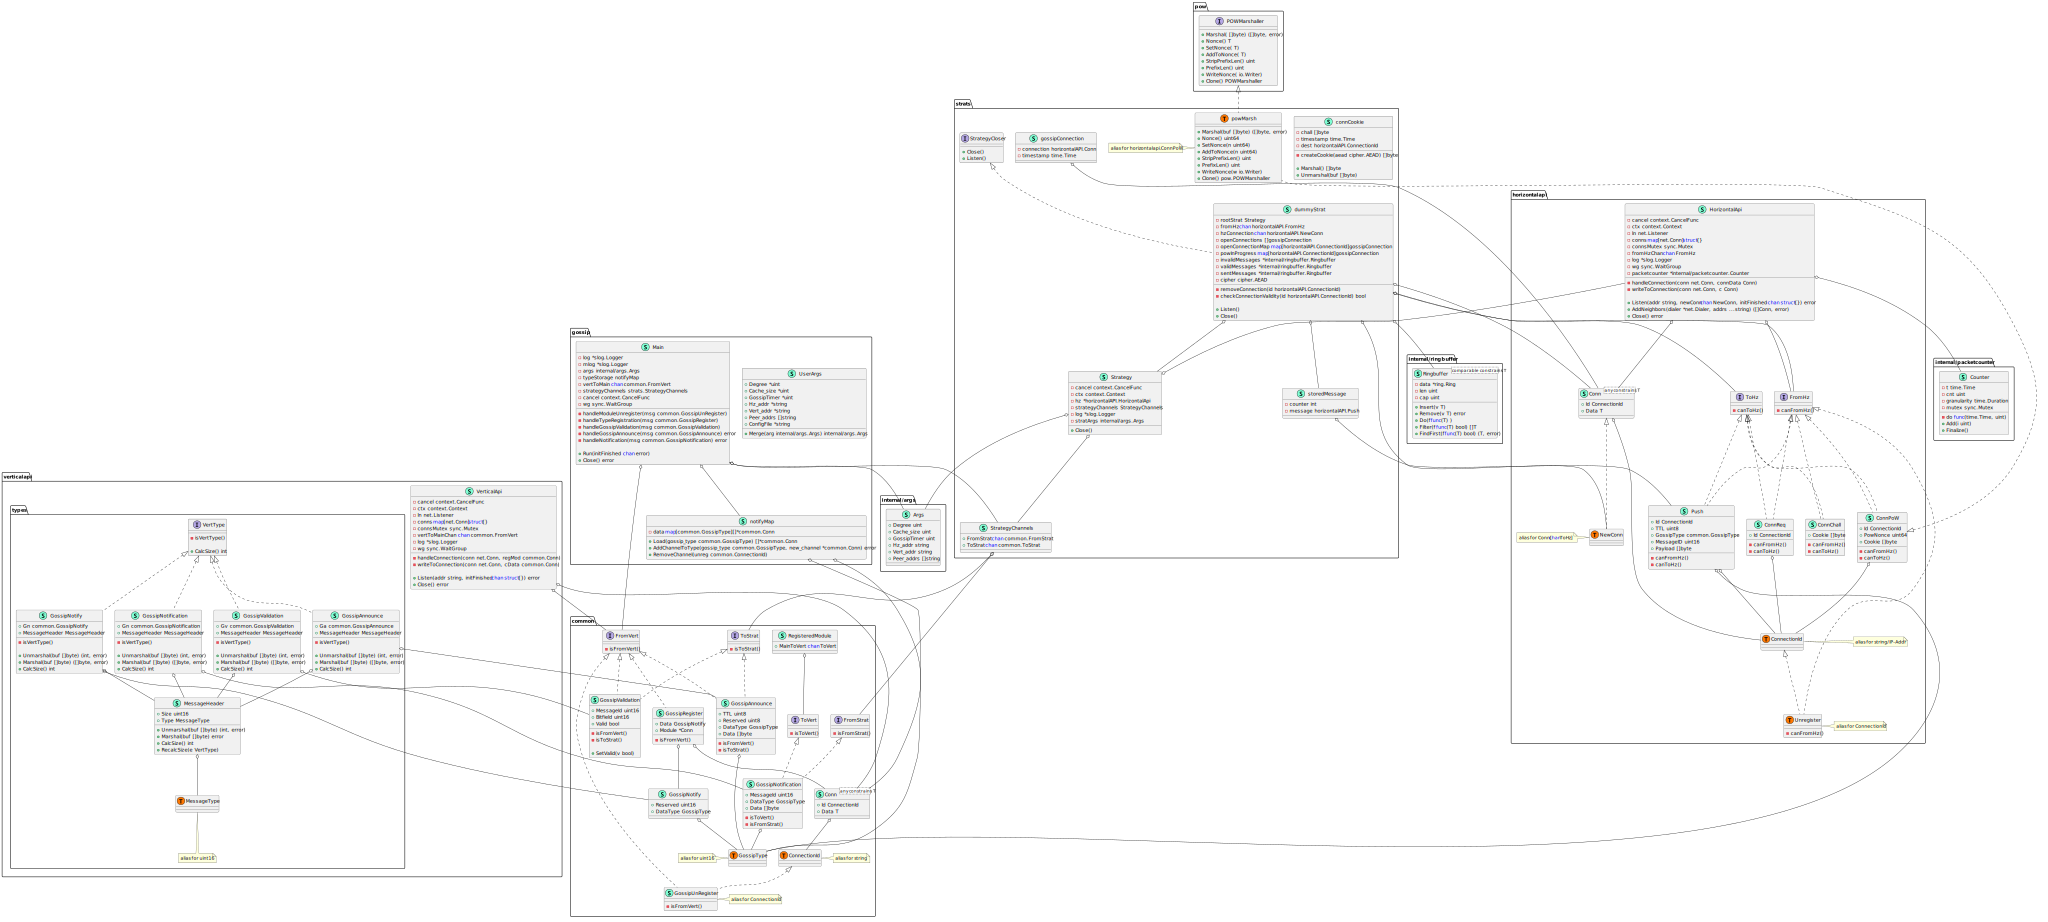
\includegraphics[width=1.2\linewidth]{figures/class}
		\caption{Class diagram.}
		\label{fig:class:dia}
	\end{figure}
\end{landscape}

\subsection{Process architecture}
% TODO(Fabio)

\Todo{come up with scenario (reg, announce \quad|\quad notify > validation) to explain message-passing}
\Todo{figure for message types on different channels}

\begin{figure}
	\centering
	\begin{messagepassing}
	\newprocesswithlength{main}{4}
	\newprocesswithlength{vertAPI}{4}
	\sendwithname{main}{1}{vertAPI}{2}{msg}
\end{messagepassing}

	\caption{Messagepassing of one instance/scenario.}
	\label{fig:msg}
\end{figure}

% \begin{figure}
% 	\centering
% 	\begin{tikzpicture}[automata]
	\node[state, initial,initial text={new mID}] (inv) {invalid};
	\node[state,accepting,right=of inv] (val) {valid};
	\node[state,right=of val] (sent) {sent};
	\node[state,below=of val] (del) {deleted};
	%
	\path (inv) edge[->] node[sloped,above] {valid=True} (val);
	\path (val) edge node[sloped,above] {sent x times} (sent);
	%
	\path (inv) edge[bend right=10] node[sloped,below] {valid=False} (del);
	\path (inv) edge[bend left=10] node[sloped,above] {cache full} (del);
	\path (val) edge node[sloped,above] {cache full} (del);
	\path (sent) edge node[sloped,above] {cache full} (del);
\end{tikzpicture}

% 	\caption{Finite state machine for message caching.}
% 	\label{fig:fsm_msgs}
% \end{figure}

threading, multi-process, ... (a lot of intersection with the classes, but I think here we can go in depth about the communication part)

\subsection{Networking} 
% TODO(Lukas)

\Todo{vertAPI (ser/deserialization) and horAPI (capnproto)}

\section{Security Measures}
% TODO(Fabio)

\Todo{not in place, but put some thought into it (PoW for participation) \tos \cf future work}

E.g secure channels between peers, sybil resistance mechanism, concurrent lookup paths in DHT protocol, . . . 

You should briefly describe the intention behind the security measure and how you want to implement it


\section{Specification of the peer-to-peer protocol}
% TODO(Lukas)

(that will be implemented)

Message formats (as given in this document)

Reasoning why the messages are needed

\subsection{capnproto}
\subsubsection{push}
\begin{table}
	\centering
	\begin{tabularx}{.85\linewidth}{llX}
	\toprule
	Field & Type & Description
	\\
	\midrule
	ttl & Uint8 & Time to live: specifies nodes until which distance to the transmitting node should be reached ($\text{TTL} = 0 \text{ means } \infty$)
	\\
	gossipType & Uint16 & Type of the payload (set by the module talking on the verticalAPI)
	\\
	messageID & Uint16 & Identifier of this message (randomely chosen by the strategy)
	\\
	payload & Data & Bytes of data that is spread in the network
	\\
	\bottomrule
\end{tabularx}

	\caption{Contents of a push packet.}
	\label{tab:push}
\end{table}
See \cref{tab:push} for reference.

\section{Future Work}
% TODO(Lukas)

\Todo{e2e testing, more strategies (like pull), \enquote{benchmarking}, \cf security measure}
\Todo{see meeting3.md}

Features you wanted to include in the implementation but couldn’t finish so far

\section{Workload distribution}

% TODO(Fabio)
\Todo{Fabio: strategy (peeer programming), vertAPI (testing), main (both)}

% TODO(Lukas)
\Todo{Lukas: horAPI, vertAPI -> common (code, copy-paste from regClient), main (both)}


\todos

\end{document}
